%%%%%%%%%%%%%%%%%%%%%%%%%%%%%%%%%%%%%%%%%%%%%%%%%%%%%%%%%%%%%%%%%%%%
\section{Overview}
\label{sec:fd-daq-ov}

\metainfo{Georgia Karagiorgi and Dave Newbold. 2 Pages - largely
  generic but some highlighting of SP-specifics. 
  Focus on describing to HEP but non-DAQ expert. 
  Include how design is resilient in the face of potential
  uncertainties such as excess noise or the need to reduce drift HV
  (just two examples, maybe there are more).}

%%%%%%%%%%%%%%%%%%%%%%%%%%%%%%%%%
\subsection{Introduction}
\label{sec:fd-daq-intro}

The DUNE \dword{fd} \dword{daq} system design must enable the
readout, triggering, processing and distribution to permanent storage
of data from all \dwords{detmodule} which includes both their
electrical \dword{tpc} and optical \dword{pds} signals. 
The \dwords{detmodule} have variation in terms of their readout
technology and schemes, timing system, channel counts and data
throughput and format. 
The DAQ must adapt to these differences at its front end such that a
high degree of design commonality can be reused between
\dwords{detmodule} and to present a unified interface to the consumer
of its data at its back end.
It must also accept and process the data from a variety of other
sources including the accelerator, various calibration systems
(including laser, cold electronics, photodetectors, and potentially
others) as well as trigger sources external to DUNE.  

The DUNE physics program requires that the detector is highly
sensitive to both beam and off-beam events.
The latter include most dominantly cosmic rays and atmospheric
neutrino interactions, as well as hypothesized, rare interactions such
as nucleon decay, other baryon number violating signatures (such as
neutron-antineutron oscillation), and interactions from nearby
\dwords{snb}. 
Beam interactions and off-beam high-energy interactions pose
relatively little challenge to the DAQ system.
In the former case triggering can be done with the benefit of
information on the beam timing from the accelerator and in the latter
case the presence of large, localized activity in the detector, seen
by both the \dword{tpc} and \dword{pds}. 
On the other hand, the low activity and extended nature (both
spatially and in time) of neutrino events from a supernova burst,
compounded, on one hand, with the overall large data rates of the DUNE
far detector and, on the other hand, naturally occuring radiological
backgrounds which have similar activity as low-energy supernova
neutrino interactions, pose a huge challenge to the \dword{daq}.
As such, the \dword{daq} and in particular the far detector trigger
scheme is being designed with that challenge in mind. 

\begin{dunefigure}[DAQ Overview]{fig:daq-cartoon}{DUNE FD DAQ readout scheme.}
  \begin{center}
    t.b.d
  \end{center}
\end{dunefigure}

Figure~\ref{fig:daq-cartoon} provides a cartoon picture for the DUNE
far detector readout scheme.
One particular concern is the optimal method of reducing the data
volume from the \dwords{tpc}.
Their excess electronics noise and uncertainties in the rates of
radiological decay pose a risk in grossly underestimating the rate of
data associated with low-energy physics.
Rather than relying on smart zero-suppression or other waveform-level
lossy schemes, which are far more sensitive to noise and radiological
rate fluctuations, the approach followed by the \dword{daq} design has
been to facilitate as efficient and effective triggering as possible,
coupled with lossless readout.
The figure illustrates the readout scheme for localized high-energy as
well as extended low-energy events.


\begin{dunefigure}[DAQ Overview]{fig:daq-overview}
  {The high-level design for the DUNE FD DAQ showing data (solid, with
    line width indicating throughput) and trigger (dashed) flows. 
    A detector module has specialized implementation of some of these
    high level components, particularly toward the upstream front-end
    as described in the text. 
    The grayed boxes are not in the DAQ scope.
    See text for details.
}
% This PDF is made from the .dot of the same name.
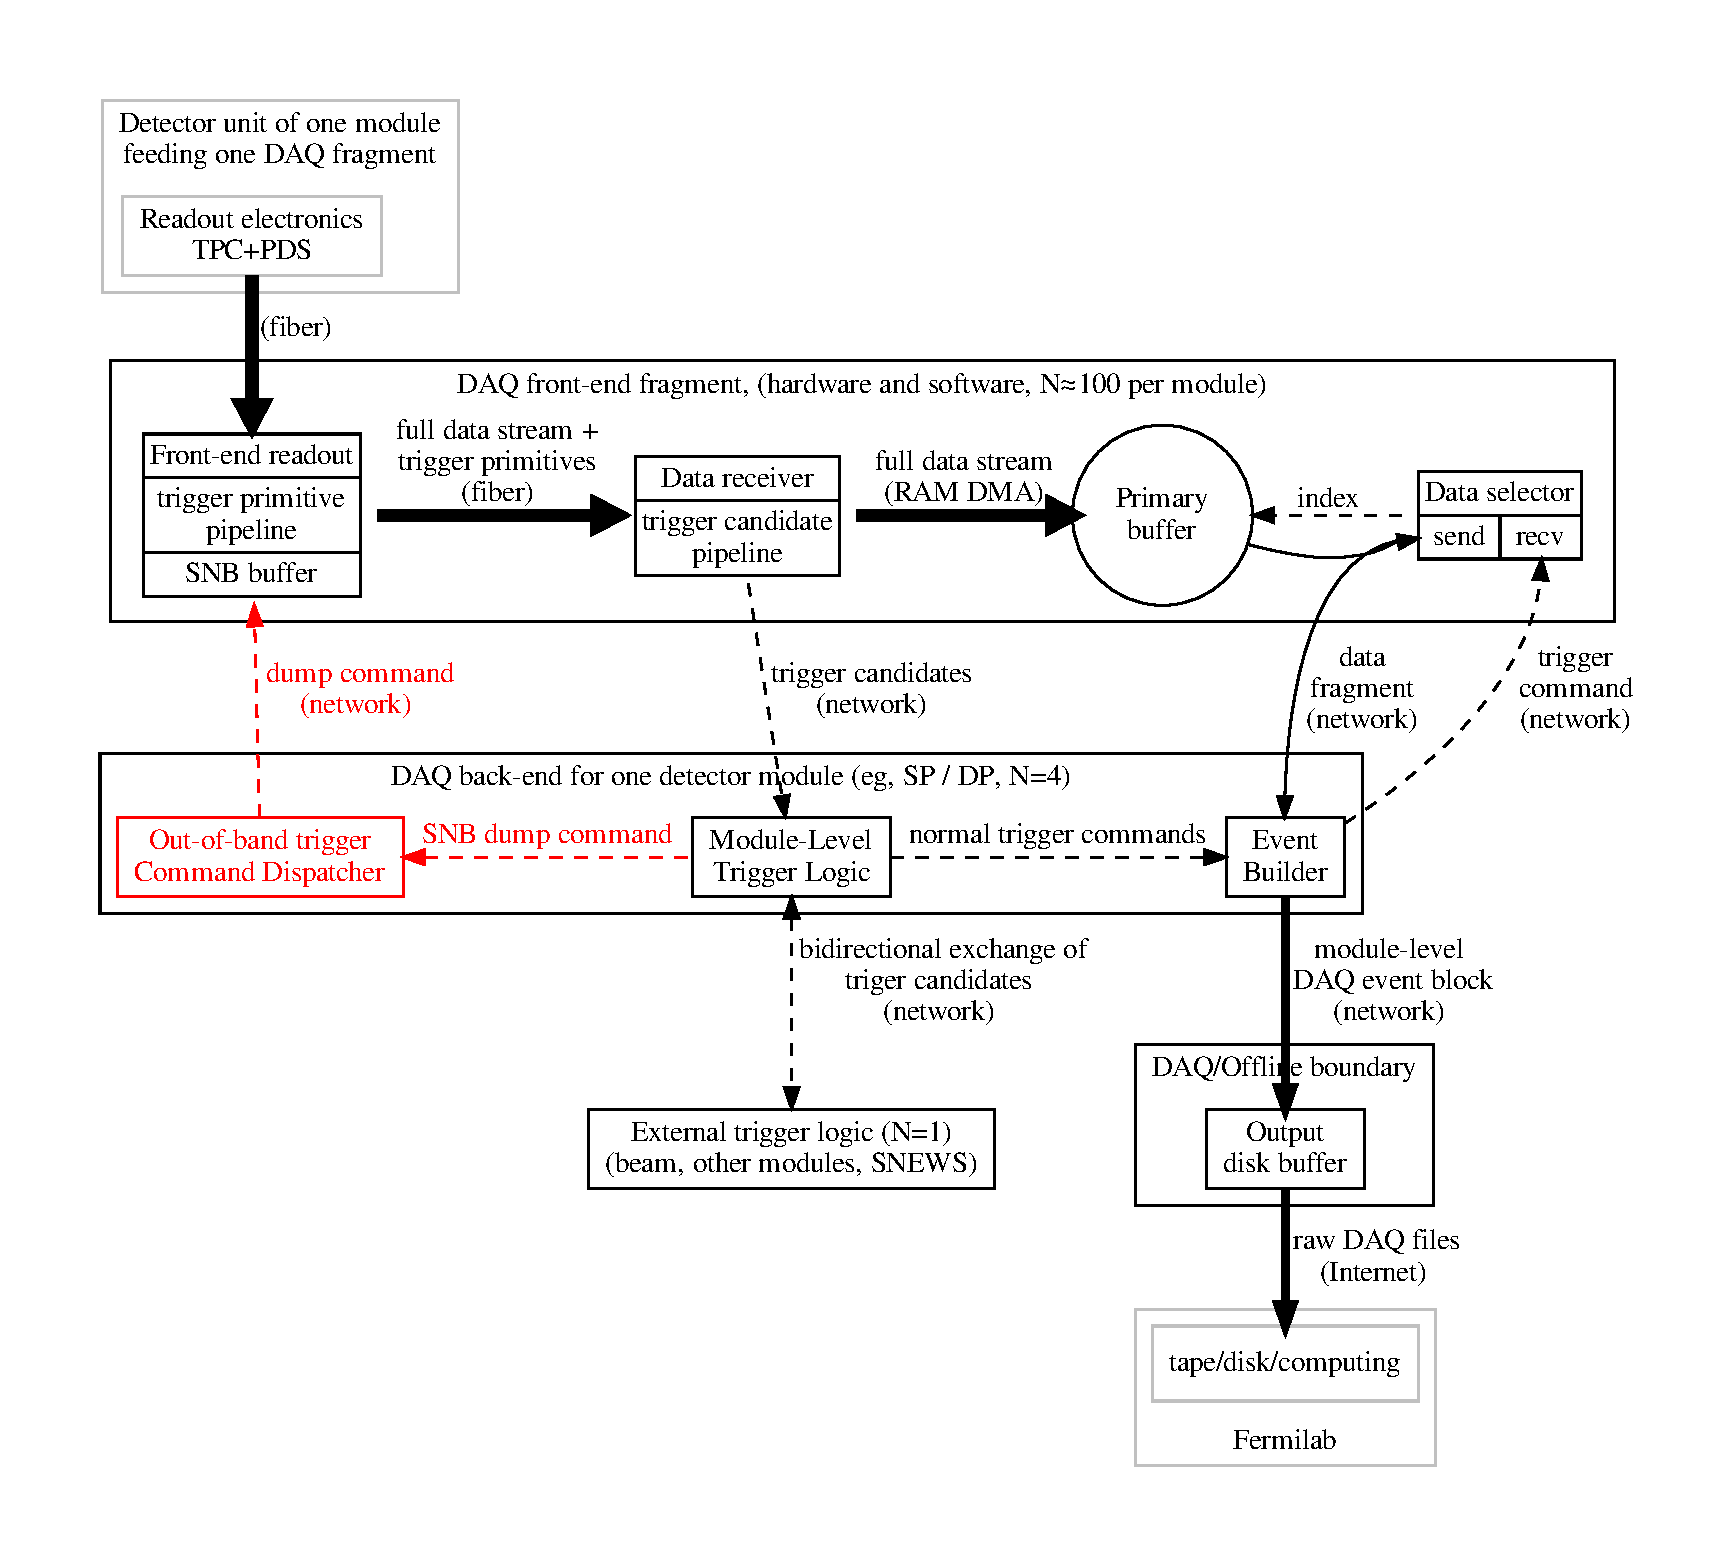
\includegraphics[width=0.8\textwidth]{high-level-daq.pdf}%
\end{dunefigure}


Figure~\ref{fig:daq-overview} gives an illustration of the high-level
DUNE FD DAQ design in terms of data and trigger flow.
At this level, the design is generic to all \dwords{detmodule}.  
The implementation some of the upstream components necessarily differ
in order to match differences in the design of the detector module
itself. 
The design section below gives more description of this high-level
design and details on specialized implementations.



%%%%%%%%%%%%%%%%%%%%%%%%%%%%%%%%%%%%%

\subsection{Design Considerations}
\label{sec:fd-daq-des-consid}

\fixme{Start with a statement about the different physics requirements and corresponding challenges for DAQ, and potentially an overview of the solutions.  Eg. beam events can be collected using local trigger \& readout, or at module level (eg. during commissioning), SNB requires global trigger \& readout, etc.}
%\metainfo{Include: Raw data rate from WIBs, Josh's table of data volumes for each event type and the 30 PB/year offline limit. Space and thermal power limits.  Note, this table may be better put into Section~\ref{sec:fd-daq-design} to make this section more generic.}

%\fixme{Anne suggests: Within this section add ref to requirements
%document when it's ready, and maybe list the most important half
%dozen in a table here). E.g.,}  
The high level requirements for the DUNE FD DAQ are provided in
\cite{daq:reqs}.
The most critical requirements in consideration for the overall design
are summarized in Table~\ref{tab:daqrequirements}.

\begin{dunetable}[Important requirements on the DAQ system design]
{p{0.2\textwidth}p{0.6\textwidth}}
{tab:daqrequirements}
{Important requirements on the DAQ system design}   
Requirement  & Description \\ \toprowrule
Scalability & The DUNE FD DAQ shall be capable of receiving and
buffering the full raw data from all four FD modules \\ \colhline 
Zero deadtime & The DUNE FD DAQ shall operate without deadtime under
"normal" operating conditions \\ \colhline
Triggering & The DUNE FD DAQ shall provide full-detector triggering
functionality as well as self-triggering
functionality; the data selection shall maintain high efficiency to
physics events while operating within a total bandwidth of 30 PB/year
for all operating FD modules \\ \colhline
Synchronization & The DUNE FD DAQ will provide synchronization of
different FD modules to within 1~$\mu$s, and of different subsystems
within a module to within 10~ns\\ \colhline
\end{dunetable}

The input bandwidth and processing needs of the DAQ are expected to be
dominated by the rate of data produced by the TPC system of each
\dword{detmodule}.
These rates vary between the modules and their estimations are summarized in
Table.~\ref{tab:daq-input-bandwidth}.
\begin{dunetable} [Pre-trigger data rates from the DUNE FD TPCs and into DAQ front end.]
  {lll} {tab:daq-input-bandwidth} {The parameters governing the pre-trigger data rate from units of each \dword{detmodule} TPC \dwords{ce} and the aggregate throughput into the \dwords{fec} of the DAQ \dwords{daqfrag}.  Compression is an estimate and will be reduced if excess noise is introduced.  
  }
  parameter & \dlong{sp} & \dlong{dp} \\
  \colhline
  TPC unit & APA & CRO crate \\
  unit multiplicity & 150 & 240 \\
  channels per unit & 2560 (800 collection) & 640 (all collection) \\
  ADC sampling & \SI{2}{\MHz} & \SI{2.5}{\MHz} \\
  ADC resolution & 12 bit & 12 bit \\
  \colhline
  aggregate from \dword{ce} & \SI{1440}{\GB/\s} & \SI{576}{\GB/\s} \\
  compression factor & 5$\times$ (in \dshort{daqfer}) & 10$\times$ (in \dshort{cro} crate) \\
  aggregate to FEC & \SI{230}{\GB/\s} & \SI{58}{\GB/\s} \\
  \colhline
\end{dunetable}

The ultimate limit on the output data rate of the DUNE FD DAQ is
expected to be provided by the available bandwidth to and the tape,
disk and processing capacity of Fermilab. 
An ample guideline has been established which places this limit at
about \offsitepbpy or \offsitegbps.
Extrapolating to four FD detector modules this requires the DAQ to
perform a data reduction factor of more than \num{4000}. 
How this is achieved is described next.

An overestimate of the annual, triggered data volume assuming the FD
is comprised of four \dword{sp} \dwords{detmodule} is summarized in
Table.~\ref{tab:daq-data-rates}. 
It assumes a very generous and simple trigger scheme whereby the data
from the entire \dword{detmodule} is saved for a period longer than
two drift times around the trigger time.
This essentially removes selection bias at the cost of producing
substantially more data.
It is important to note that as generous as this scheme is, the
overestimate meets the required data reduction factor described above.  
It is expected that future studies, including early data taking, will
discover ways to reduce the data volume while retaining high selection
efficiency and low bias.

\begin{dunetable}
[Anticipated event and data rates assuming four SP modules.]
{p{0.25\textwidth}p{0.15\textwidth}p{0.4\textwidth}}
{tab:daq-data-rates}
{Anticipated event and data rates assuming four SP modules. The
  rates assume continuous readout (without any data reduction) for
  5.4~ms for non-extended events, and for 10 seconds for extended events.}   
Event Type  & Annual Data Volume & Assumptions \\ \toprowrule
 Beam interactions & 27 TB & 800 beam and 800 dirt muons; 10~MeV
 threshold in coincidence with beam time; include cosmics\\ \colhline
 Cosmics and atmospherics & 10 PB &  \\ \colhline
 Radiologicals & $\le$1~PB & fake rate of $\le$100 per year \cite{daq:simreport}\\ \colhline
 Front-end calibration & 200~TB & Four calibration runs per year, 100
 measurements per point \\ \colhline
 Radioactive source calibration & 100~TB & source rate $\le$10~Hz;
 single APA readout; lossless readout \\ \colhline
 Laser calibration & 200~TB & 1$\times$10$^6$ total laser
 pulses, lossy readout \\ \colhline
 Random triggers & 60 TB & 45 per day\\ \colhline
 Trigger primitives & $\le$6~PB &  all three wire planes; 12 bits per
 primitive word; 4 primitive quantities; $^{39}$Ar-dominated\\ \colhline
\end{dunetable}


It assumes the level of noise is consistent with the expected,
intrinsic, thermal noise of the electronics.
Trigger rates increase and compression factors decrease in a manner
that is sensitive to the amount and type of excess noise, such as can
be due to \dword{rf} emission inside the cryostat. 
Future studies may be done over a variety of guesses for different
possible excess noise scenarios and they will receive beneficial input
from the results of \dword{protodune}.

\fixme{Table~\ref{tab:daq-data-rates} is really unclear.  Need to clarify the physical origin, trigger and readout type for each one. Assumptions also include quite a bit of jargon.}

\fixme{Table~\ref{tab:daq-data-rates} - 10s for extended events is out of date. What are we saying ?}

\fixme{Table~\ref{tab:daq-data-rates} does not include 5x compression, right?  If not, it should be adjusted to include it.}

\fixme{Table~\ref{tab:daq-data-rates} should add SNB data.}

\fixme{Table~\ref{tab:daq-data-rates}, caption and text should maybe divide by 4 and say it's just SP.  We can have a summary statement where we extrapolate to SP+DP+M3+M4.}




%%%%%%%%%%%%%%%%%%%%%%%%%%%%%%%%
\subsection{Scope}
\label{sec:fd-daq-scope}

%\metainfo{This section may also wish to refer to Fig.~\ref{fig:daq-overview}.}

The scope of the \dword{daq} system is illustrated in
Fig.~\ref{fig:daq-overview} by the boxes which are not grayed out and
includes the continued procurement of materials for, and the
fabrication, testing, delivery and installation of the following
systems:

\begin{itemize}
\item Front-end readout hardware and firmware/software development for \dword{trigprimitive} generation.
\item Front-end computing for hosting of \dword{daqdr}, \dword{ringbuffer} and \dword{daqds}.
\item Back-end computing for hosting \dword{mtl}, \dword{eb} and the \dword{daqoob} processes.
\item External trigger logic and its host computing.
\item Algorithms to generate trigger commands which perform data selection.
\item Timing distribution system
\item DAQ data handling software including receiving and building of
  events
\item Run control software, configuration database, and user interface
\item Rack infrastructure in the central utility cavern for readout
  electronics, front-end computing, timing distribution, and data
  selection
\item Rack infrastructure on surface at SURF for back-end computing
\end{itemize}


